\documentclass[a4paper,12pt]{article}
\usepackage{titling}
\usepackage[OT4]{fontenc}
\usepackage[english,polish]{babel}
\usepackage{amsmath, amsfonts, amsthm, latexsym}
\DeclareRobustCommand{\sqbullet}{%
	\raisebox{.3ex}{\rule{.3em}{.3em}}%
}
% Margins in document
%\usepackage[left=2.5cm, right=2.5cm, top=3.5cm]{geometry}

% Indentation at the beginning of chapters/sections
\usepackage{indentfirst}

% Ceiling functions
\usepackage{mathtools}
\DeclarePairedDelimiter{\ceil}{\lceil}{\rceil}

% Avoid  colons before tables' empty captions and change caption
\usepackage{caption}
\captionsetup[table]{name=Tab.}
\captionsetup[figure]{name=Rys.}

% Don't know why, it starts from 2
\addtocounter{table}{0}

% Rename tables' suffix
\renewcommand{\tablename}{Tab.}

% Graphicx setup
\usepackage{graphicx}
\graphicspath{{graphics/}{../graphics/}}

% No separator between items
\usepackage{enumitem}
\setlist{nolistsep}

% Pagebreak before every \section
\let\oldsection\section
\renewcommand\section{\clearpage\oldsection}

% Bigger padding in tabulars
\usepackage{array}
\setlength\extrarowheight{3pt}

%\usepackage{amssymb}
\usepackage{algorithm}
\usepackage{algorithmic}
\usepackage{amsmath}

\PassOptionsToPackage{hyphens}{url}\usepackage{hyperref}

% Itemize in tabulars (avoid big margins with minipage)
\newcommand{\tabbeditemize}[1]{
	\begin{minipage}[t]{0.4\textwidth}
		\begin{itemize}[topsep=0mm,partopsep=0mm,leftmargin=4mm]
			#1
		\end{itemize}
\end{minipage}}

% listings
\usepackage{xcolor}
\usepackage{listings}
\usepackage{hyperref}
\usepackage{pdfpages}
\definecolor{codegreen}{rgb}{0,0.7,0}
\definecolor{codegray}{rgb}{0.5,0.5,0.5}
\definecolor{codepurple}{rgb}{0.58,0,0.82}
\definecolor{backcolour}{rgb}{0.95,0.95,0.92}
\lstdefinestyle{mystyle}{
	language=Python,
	deletekeywords={from},
	backgroundcolor=\color{backcolour},   
	commentstyle=\color{codegreen},
	keywordstyle=\color{magenta},
	numberstyle=\tiny\color{codegray},
	stringstyle=\color{codepurple},
	basicstyle=\ttfamily\footnotesize,
	breakatwhitespace=false,         
	breaklines=true,                 
	captionpos=b,                    
	keepspaces=true,                 
	numbers=left,                    
	numbersep=5pt,                  
	showspaces=false,                
	showstringspaces=false,
	showtabs=false,                  
	tabsize=4
}
\makeatletter
\newcommand*{\toccontents}{\@starttoc{tableofcontents}}
\makeatother


% DOCUMENT
\title{Sprawozdanie \\
\Large Zastosowanie uczenia maszynowego do gry wyścigowej}

\author{Mateusz Burczaniuk,\\ Patryk Fijałkowski}


% ============================================
% CONTENT ====================================
% ============================================

\begin{document}
	\maketitle
	%\vspace{3cm}
	\tableofcontents

\section{Wprowadzenie}
\subsection{Problem}
Omawiana gra wyścigowa symuluje rywalizację na torze pomiędzy kilkoma samochodami wyścigowymi. Tor, na którym odbywa się rywalizacja jest zamkniętą pętlą otoczoną niezbyt wysokimi ścianami. Poza tym na torze występują także przeszkody. Samochód może poruszać się do przodu, do tyłu, skręcać w~lewo, prawo lub wykorzystać nitro. Zderzenie samochodu gracza ze ścianą lub przeszkodą powoduje natychmiastową śmierć gracza i~koniec gry. Zderzenie dwóch graczy ze sobą powoduje analogiczne skutki (śmierć i~usunięcie z~rozgrywki) dla obu graczy.

Gracz ma zadanie przejechać zadaną trasę jak najszybciej, wyprzedzając swoich rywali. Podczas rywalizacji gracz może znacznie zwiększyć swoją prędkość przy użyciu nitro. Jednak maksymalna dostępna w~danej chwili ilość nitro jest ograniczona, więc gracz nie może używać go bez przerwy. Zużyte nitro stopniowo odnawia się i~po pewnym czasie wraca do pierwotnego poziomu. Może ono odnawiać się nieskończoną liczbę razy.

Wszystkie rozważane pojazdy mają taki same parametry techniczne i~osiągi, w~związku z~czym wygrana lub przegrana w~wyścigu zależy wyłącznie od obranego przez nie sposobu przemieszczania się po torze.

Zatem postawiony problem składa się z~kilku zagadnień - należy zoptymalizować politykę doboru kierunku poruszania się gracza oraz używania nitro tak, aby przejechać całą trasę bez żadnego zderzenia, a~jednocześnie jak najszybciej, pozostawiając rywali za sobą. Zadania te w~pewnym stopniu konfliktują ze sobą, gdyż optymalną strategią w~celu uniknięcia zderzeń jest stanie w~miejscu, natomiast dążenie do uzyskania optymalnego czasu przejazdu powoduje wzrost ryzyka zderzenia z~przeszkodą lub innym pojazdem.


\subsection{Stan wiedzy}

Omawiany problem reprezentuje zagadnienie kontroli w~ciągłej przestrzeni stanów. Istnieje kilka sposobów rozwiązywania tego typu problemów. Do czołowych algorytmów w~tej dziedzinie należą obecnie zarówno metody on-policy, jak i~off policy. W~niniejszej pracy w~kontekście omawianego zadania przetestowano dwie stosunkowo młode metody, ale znacznie różniące się metody: PPO oraz SAC.

\subsection{Użyte technologie}
Prezentowane rozwiązanie zostało wykonane w silniku Unity w wersji 2019.4.11f1. Wykorzystano również framework ml-agents w wersji 0.21.1, odpowiedzialny za proces uczenia agentów.

\subsection{PPO}
Proximal Policy Optimization, czyli PPO to nowa metoda, wprowadzona w~2017 roku. Wykorzystuje ona metodę aktor- krytyk, posługując się dwoma sieciami neuronowymi. Aktor jest reprezentowany przez sieć neuronową, która wykonuje zadanie klasyfikacji, wybierając, jaką akcję podjąć przy obserwowanym stanie środowiska. Krytyk to druga sieć, o~podobnej strukturze, która uczy się oceniać, czy poszczególne akcje poprawiają, czy pogarszają stan. Krytyk zwraca Q-wartość akcji wybranej w~poprzednim stanie. Na tej podstawie aktor modyfikuje swoją politykę, dbając, by nie przeprowadzić zbyt dużych zmian.

W~metodzie PPO aktualna polityka wykorzystywana jest do przeprowadzenia pewnej liczby doświadczeń (wielkość tę określa się mianem rozmiaru batcha) wymagających interakcji ze środowiskiem, które wykorzystywane są do poprawy polityki. Jest to uczenie on-policy, jako, że zebrane dane są wykorzystywane tylko raz.

Algorytm korzysta z~mechanizmu Uogólnionej Estymacji Przewagi (ang. \textit{Generalized Average Estimation}), aby ustalić, które akcje przyniosły, jakie skutki. Liczona jest ona od ostatnich wykonywanych akcji. Obliczane są kolejno wartości:

\begin{equation}
	\delta = r_t + \gamma V(s_{t+1})m_t - V(s_t)
\end{equation}

\begin{equation}
	gae_t = \delta + \gamma \lambda m_t gae_{t+1}
\end{equation}

\begin{equation}
	R_t(s_t,a_t) = gae_t + V(s_t)
\end{equation}

gdzie:
\begin{itemize}
	\item $t$ - numer kroku analizowanego testu,
	\item $s_t$ - stan w chwili $t$,
	\item $a_t$ - akcja podejmowana w~chwili $t$,
	\item $V(s)$ - wartość stanu $s$,
	\item $r_t$ - nagroda w~chwili $t$.
	\item $m_t$ - maska w~chwili $t$, jeśli w~stan $t$ jest końcowy, to 0, w~przeciwnym wypadku 1.
\end{itemize}

Wystąpiły tutaj dwa hiperparametry algorytmu:
\begin{itemize}
	\item $\gamma$ - parametr dyskontowy, standardowo 0.99,
	\item $\lambda$ - parametr wygładzający, standardowo 0.95.
\end{itemize}

Wyliczane jest ratio, które mówi, jak bardzo polityka uległa zmianie.
\begin{equation}
	ratio = \pi_{new} / \pi_{old}
\end{equation}
Polityka jest oceniana przez aktora i~krytyka. Ocena krytyka to błąd średniokwadratowy pomiędzy wartością zwracaną a oszacowaniem krytyka.
\begin{equation}
	critic\_loss = (R - V(s))^2
\end{equation}

Natomiast błąd aktora wyraża się wzorem:
\begin{equation}
	actor\_loss = min(ratio * advantage, clip(ratio, 1-\varepsilon,1+\varepsilon)* advantage)
\end{equation}

$\varepsilon$ to parametr obcinania, który zapewnia, że jednorazowo zmienimy politykę o~co najwyżej $\varepsilon\%$. Domyślna wartość tego parametru wynosi 0.2.

Ostatecznie ocena polityki wyraża się wzorem:
\begin{equation}
	total\_loss = critic\_loss * critic\_discount + actor\_loss - entropy
\end{equation}

$critic\_discount$ to współczynnik mający na celu zrównoważenie wpływu na wynik oceny aktora i~oceny krytyka. Entropia to natomiast hiperparametr metody, który domyślnie przyjmuje wartość 0.005. 

Na podstawie powyższych funkcji oceny używane sieci uczone są przy użyciu metody stochastycznego przyrostu gradientu. Sieć jest uczona na danych z~pojedynczego batcha przez pewną liczbę epok, będącą hiperparametrem metody.

Opis działania metody PPO został oparty na artykułach C. Trivediego \cite{ppo1},\cite{ppo2}.


\subsection{SAC}
Soft Actor-Critic, czyli SAC to też stosunkowo nowa metoda do rozwiązywania tego typu problemów. W~przeciwieństwie do PPO jest to metoda off-policy, czyli wyniki uzyskane przy użyciu jednej polityki są wykorzystywane do oceny następnych polityk.

Algorytm ten modyfikuje funkcję celu, aby maksymalizować nie tylko nagrody, ale również entropię polityki, aby wspierać eksplorację przestrzeni stanów. Funkcja ta jest zdefiniowana następująco:

\begin{equation}
	J(\pi) = \sum_{t=0}^T \mathbb{E}_{(s_t,a_t) \sim \rho_\pi} [r(s_t,a_t) + \alpha H(\pi(\cdot |s_t))]
\end{equation}

$\alpha$ to parametr, który określa wagę entropii.

SAC używa trzech sieci neuronowych:
\begin{itemize}
	\item określającej wartość stanu V z~parametrem $\psi$,
	\item określającej funkcję Q z~parametrem $\theta$,
	\item określającej funkcję polityki z~parametrem $\phi$.
\end{itemize}

Sieć V jest uczona tak, aby zminimalizować błąd  kwadratowy pomiędzy predykcją wartości zwracanej przez sieć a wartością oczekiwaną sumy funkcji Q i~entropii:

\begin{equation}
J_V(\psi) = \mathbb{E}_{s_t \sim D}\Big[ \frac{1}{2}\big(V_\psi(s_t) - \mathbb{E}_{a_t \sim\pi_\phi} [Q_\theta(s_t,a_t) - log \pi_\phi (a_t|s_t)] \big)^2\Big]
\end{equation}

Sieć Q minimalizuje błąd średniokwadratowy pomiędzy predykcją funkcji Q a natychmiastową nagrodą zsumowaną ze zdyskontowaną predykcją wartości następnego stanu.

\begin{equation}
	J_Q(\theta) = \mathbb(E)_{(s_t,a_t) \sim D}\Big[
		\frac{1}{2} \big(
			Q_\theta(s_t,a_t) - r(s_t,a_t) - \gamma \mathbb{E}_{s_{t+1 \sim p}}[V_{\bar{\psi}}(s_{t+1})]
		\big)
	\Big]
\end{equation}

Sieć $\pi$ ma za zadanie minimalizować różnicę pomiędzy wartością zwracaną przez sieć  a~wartością $\frac{exp(Q_\theta(s_t,\cdot))}{Z_\theta(s_t)}$, gdzie Z to funkcja normalizująca. Matematyczny opis tej zależności wykorzystuje dywergencję Kullbacka-Leiblera i~można go przedstawić przy użyciu wzoru:

\begin{equation}
	J_\pi(\phi) = \mathbb(E)_{s_t \sim D}\Big[ D_{KL} \big(\pi_\phi(\cdot|s_t) || \frac{exp(Q_\theta(s_t,\cdot))}{Z_\theta(s_t)}  \big) \Big]
\end{equation}

Przy wyliczaniu tej wartości używana jest też pewna technika reparemetryzacji.



Schemat algorytmu przedstawiono na Listingu \ref{alg:sac}.
\begin{algorithm}[h!]
	\caption{SAC}
	\label{alg:sac}
	\begin{algorithmic}[1]
		\STATE $\psi, \bar{\psi}, \theta,\phi$ - dane parametry
		\FOR {$i=0,\dots,max\_iteration$}
			\FOR {ruch środowiska}
				\STATE $a_t \sim \pi_{\phi}(a_t|s_t)$
				\STATE $_{t+1} \sim p(s_{t+1}|s_t,a_t)$
				\STATE $D \gets D \cup \{(s_t,a_t,r(s_t,a_t),s_{t+1})\}$
			\ENDFOR
		\ENDFOR
		\STATE Popraw parametry sieci przy użyciu gradientów poszczególnych funkcji dopasowania.
	\end{algorithmic}
\end{algorithm}

Opis algorytmu sporządzono w oparciu o~artykuły \cite{kumar},\cite{nieznany}.

\section{Eksperymenty}
Przeprowadzone testy podzielono na dwie fazy. Pierwsza ma za zadanie określić najlepsze środowisko i zasady uczenia dla agentów. Z kolei druga faza skupia się na dobraniu jak najbardziej optymalnych parametrów w metodach PPO i SAC. W fazie pierwszej agenci byli uczeni do 100000 kroków, a w przypadku fazy drugiej -- do 200000 kroków.

Za ocenę każdego z nauczonych modeli przyjęto dwie miary: $k, u$. Każda z miar mieści się w zakresie $[0,1]$ i ma ocenić skuteczność wyuczonego modelu w różnych warunkach. Obie miary to stosunek średniej liczby przejechanych punktów kontrolnych (po 50 podejściach agenta do wyścigu) do pewnej empirycznie ustalonej wartości. W każdym z podrozdziałów wartość była inna, co dało możliwość znormalizowania wyników i w konsekwencji przejrzystszą ich analizę.
\begin{itemize}
	\item Miara $k$ (ang. \textit{known}) - określa, jak dobrze model radzi sobie na torze, na którym przebiegało uczenie.
	\item Miara $u$ (ang. \textit{unknown}) - określa, jak dobrze model radzi sobie na nowym torze. 
\end{itemize}


\subsection{Faza pierwsza}
\subsubsection{Wypłaty}
Sprawdzono różne podejścia nagradzania agentów. Trzy zasadnicze podejścia do udzielania wypłat:
\begin{itemize}
	\item wypłata za przejechanie punktu kontrolnego,
	\item wypłata zwiększana z czasem życia agenta,
	\item wypłata zależna od aktualnej prędkości.
\end{itemize}

W ramach zachęcenia agentów do przemierzania toru zgodnie z założeniami, na obu torach testowych umieszczono 22 punkty kontrolne. Agent w momencie przejechania przez dany punkt dostaje stałą wypłatę. Wyniki przeprowadzonych testów zostały zaprezentowane w tabeli \ref{tab:wyplaty}.

Analizując wyniki eksperymentu, zauważamy że warto wprowadzać wysokie wypłaty za punkty kontrolne, ponieważ to jednoznacznie poprawia obie miary. W przypadku nagradzania agenta za długość życia nie zauważono znaczącej poprawy w kontekście osiągów na torach testowych.

\begin{table}[H]
	\centering
	\smallskip
	\begin{tabular}{|l|l|l|l|l|}
		\hline
		Prędkość & Długość życia & Punkty kontrolne & Miara $k$ & Miara $u$ \\
		\hline
		0.15 & 0 & 10 & 1 & 0.41 \\
		0.15 & 0 & 6 & 0.64 & 0.15 \\
		0.15 & 0 & 2 & 0.68 & 0.18 \\ \hline
		0 & 0.1 & 10 & 0.47 & 0.14 \\
		0 & 0.2 & 10 & 0.52 & 0.17 \\
		0 & 0.3 & 10 & 0.55 & 0.08 \\ \hline
	\end{tabular}
	\caption{Testy wypłat}
	\label{tab:wyplaty}
\end{table}


\subsubsection{Raycasty}
Postanowiono sprawdzić wpływ liczby obserwacji odległości agenta od najbliższej przeszkody. W każdym z przypadków wysyłano raycasty z dwóch przednich narożników samochodu. Promienie były ustawione do siebie pod takim kątem, by pierwszy z nich celował z frontu samochodu, a ostatni był pod kątem $60^{\circ}$. Zgodnie z tabelą \ref{tab:raycast}, zbadano cztery możliwości -- wysyłanie odpowiednio 6, 8, 10 i 12 raycastów przez agenta.

Na podstawie uzyskanych wyników można stwierdzić, że najoptymalniej jest wysyłać 10 promieni. Zmniejszenie ich liczby do 6 i 8 nie wiąże się z istotnym pogorszeniem jakości wynikowych polityk. Jednak zwiększenie liczby promieni do 12 powoduje zauważalny spadek skuteczności agenta zarówno na torze znanym, jak i nowym.

\begin{table}[H]
	\centering
	\smallskip
	\begin{tabular}{|l|l|l|l|l|}
		\hline
		Liczba promieni & Miara $k$ & Miara $u$ \\
		\hline
		6 & 0.93 & 0.22 \\		
		8 & 0.92 & 0.33 \\		
		10 & 1 & 0.42 \\		
		12 & 0.77 & 0.21 \\\hline
	\end{tabular}
	\caption{Testy racyastów}
	\label{tab:raycast}
\end{table}


\subsection{Faza druga}
\subsubsection{PPO}
W kontekście PPO postanowiono sprawdzić wpływ parametru obcinania $\varepsilon$ oraz liczbę epok uczenia sieci neuronowej. Wyniki ukazano w tabeli \ref{tab:ppo}.

\begin{table}[H]
	\centering
	\smallskip
	\begin{tabular}{|l|l|l|l|}
		\hline
		Liczba epok & Parametr obcinania & Miara $k$ & Miara $u$ \\
		\hline
		3 & 0.1 & 0.89 & 0.32 \\		
		3 & 0.2 & 0.88 & 0.33 \\		
		3 & 0.3 & 1 & 0.37 \\		
		5 & 0.3 & 0.96 & 0.31 \\
		10 & 0.3 & 0.93 & 0.34 \\\hline
	\end{tabular}
	\caption{Testy PPO}
	\label{tab:ppo}
\end{table}

\subsubsection{SAC}
W~przypadku algorytmu SAC badano wpływ na wyniki początkowego ustawienia wartości parametru $\alpha$ związanego z~entropią. Zbadano również działanie parametru opisującego liczbę doświadczeń zbieranych do bufora przed aktualizacją polityki. Domyślnie wartość ta wynosi 0, ale powszechne jest używa się w~tym miejscu 1000 - 10000 doświadczeń. Wyniki zostały zaprezentowane w tabeli \ref{tab:sac}.

\begin{table}[H]
	\centering
	\smallskip
	\begin{tabular}{|l|l|l|l|}
		\hline
		Wartość $\alpha$ & Liczba doświadczeń & Miara $k$ & Miara $u$ \\
		\hline
		0.5 & 0 & 0.89 & 0.11 \\		
		0.7 & 0 & 1 & 0.22 \\		
		1 & 0 & 0.82 & 0.19 \\		
		0.7 & 1000 & 0.66 & 0.12 \\	
		0.7 & 10000 & 0.54 & 0.21 \\\hline
	\end{tabular}
	\caption{Testy SAC}
	\label{tab:sac}
\end{table}


\section{Obserwacje}

\subsection{Entropia}
Podczas analizy wyników zaobserwowano istotną różnice między metodami uczenia PPO i SAC. Wykres ukazujący zmiany entropii został ukazany na rysunku \ref{pic:entropy}. Dla przejrzystości zamieszczono 4 krzywe - 2 górne odpowiadają pewnym modelom metody PPO, a 2 dolne -- SAC. Zgodnie z teoretycznymi założeniami, entropia w procesie uczenia dla PPO zmniejsza się wolniej i stabilniej. 
\begin{figure}[H]
	\centering
	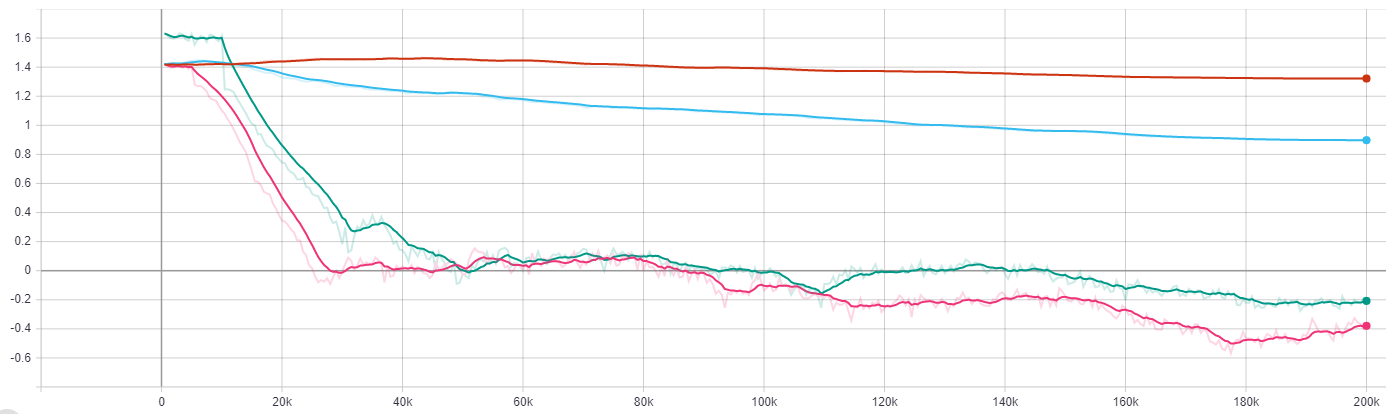
\includegraphics[width=\textwidth]{entropy}
	\caption{Entropia}
	\label{pic:entropy}
\end{figure}

\subsection{Szybkość ukończenia wyścigu}
Po przeprowadzeniu testów zauważono również, że mimo delikatnej tendencji spadkowej, średnie czasy ukończenia wyścigów w trakcie uczenia nie zmieniają się znacznie, co ukazano na wykresie z rysunku \ref{pic:szybkosc}. To oznacza, że agenci wraz z procesem uczenia nie uczą się przejeżdżać toru szybciej, a~jedynie skuteczniej omijać przeszkody, co daje im dłuższy czas życia.
\begin{figure}[H]
	\centering
	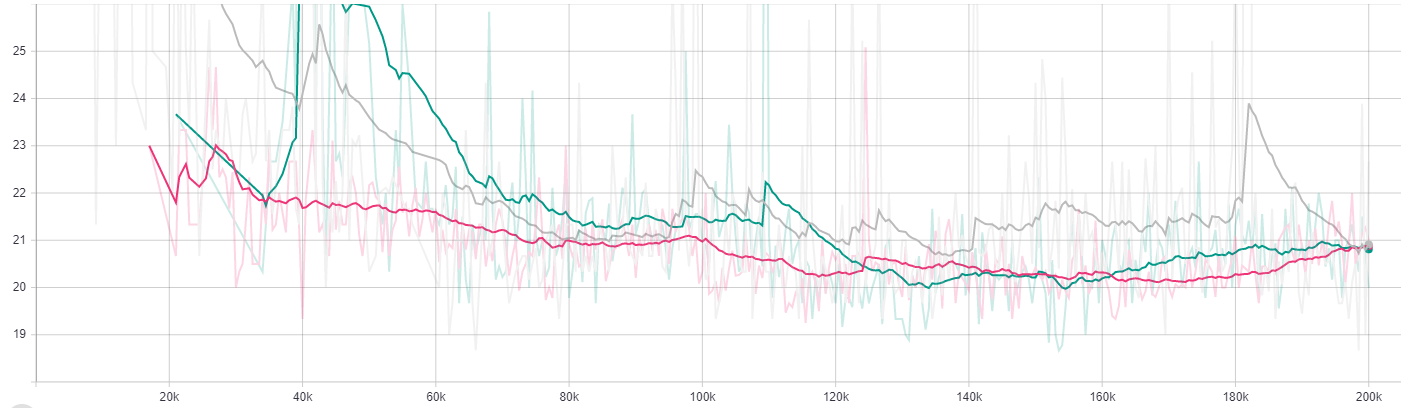
\includegraphics[width=\textwidth]{szybkosc}
	\caption{Szybkość ukończenia wyścigu}
	\label{pic:szybkosc}
\end{figure}

\subsection{Długość epizodów}
Długość epizodów uczenia w przypadku obu metod jednoznacznie rośnie, co również wykazuje poprawny charakter uczenia agentów. W przypadku metody SAC (która sprawdziła się lepiej w badanym problemie) długość epizodów rośnie szybciej i uzyskuje wartości $1.5-3$ razy wyższe. Trzy najwyższe krzywe z rysunku \ref{pic:length} odpowiadają lepszej metodzie SAC, a trzy niższe -- PPO.
\begin{figure}[H]
	\centering
	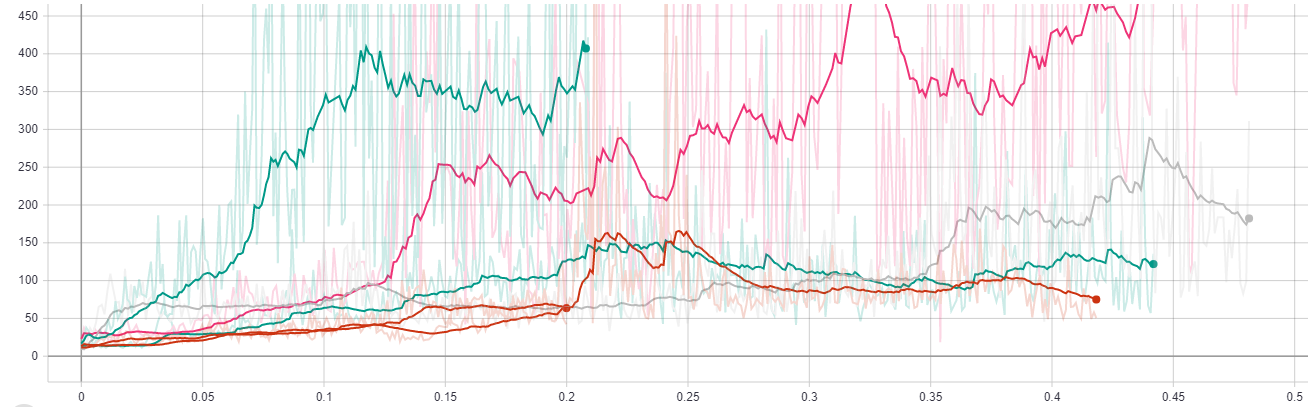
\includegraphics[width=\textwidth]{episode_length}
	\caption{Długość epizodów}
	\label{pic:length}
\end{figure}


\section{Wnioski}
Analizując wszystkie wyniki eksperymentów, zauważono że polityki utworzone metodą PPO, mimo że uzyskiwały niższe wyniki na torach, to relatywnie lepiej odnajdywały się w nowym środowisku - miały wyższą miarę $u$. Zdaje się, że agenci korzystający z polityk metody PPO ostrożniej zachowywali się na zakrętach, unikając w ten sposób kolizji z przeszkodami. W~obu przypadkach agenci podejmowali dobre decyzje w stałych fragmentach, tj. używali nitro na prostych odcinkach oraz modyfikowali tor jazdy, gdy w~zakresie widzenia pojawiały się przeszkody.

Kluczowe w kontekście narzucenia dobrego rytmu uczenia agentom było nagradzanie agentów za osiąganie kolejnych punktów kontrolnych (co wykazano w fazie pierwszej testów). Ponadto, dostosowując parametry obu metod w drugiej fazie testów można istotnie wpłynąć na proces uczenia, co przełoży się na widocznie inne polityki. Co za tym idzie, warto dostosowywać hiperparametry różnych metod, by uzyskane wyniki były jak najbardziej optymalne.

Po ukończeniu eksperymentów, ustawiono 4 najlepsze modele agentów (2 dla PPO i 2 dla SAC) do wspólnego wyścigu. Wyuczone polityki agentów pozwoliły na przeprowadzenie wyrównanych i niejednoznacznych rozgrywek. Potwierdziły się wnioski związane z dysproporcją miar $k$ i $u$ dla obu metod. Na znanym torze metoda SAC sprawdzała lepiej -- agenci korzystający z polityki wyuczonej metodą SAC jeździli ryzykowniej i lepiej wykorzystywali swoje nitro. Z kolei w nowym środowisku lepiej wypadali agenci uczeni metodą PPO -- zachowywali ostrożność w nieznanych elementach toru.

\begin{thebibliography}{20}
	\bibitem[1]{kumar}Kumar V., \textit{Soft Actor-Critic Demystified}, \url{https://towardsdatascience.com/soft-actor-critic-demystified-b8427df61665}. 2019.
	\bibitem[2]{ppo1} Trivedi C., \textit{Proximal Policy Optimization Tutorial (Part 1/2: Actor-Critic Method)}, \url{https://towardsdatascience.com/proximal-policy-optimization-tutorial-part-1-actor-critic-method-d53f9afffbf6}, 2019.
	\bibitem[3]{ppo2} Trivedi C., \textit{Proximal Policy Optimization Tutorial (Part 2/2: GAE and PPO loss)}, \url{https://towardsdatascience.com/proximal-policy-optimization-tutorial-part-2-2-gae-and-ppo-loss-fe1b3c5549e8}, 2019.
	\bibitem[4]{nieznany} \textit{SAC (soft actor-critic) algorithm for reinforcement learning}, \url{https://www.programmersought.com/article/77705189397/}
\end{thebibliography}
\end{document}
